% Copyright 2004 by Till Tantau <tantau@users.sourceforge.net>.
%
% In principle, this file can be redistributed and/or modified under
% the terms of the GNU Public License, version 2.
%
% However, this file is supposed to be a template to be modified
% for your own needs. For this reason, if you use this file as a
% template and not specifically distribute it as part of a another
% package/program, I grant the extra permission to freely copy and
% modify this file as you see fit and even to delete this copyright
% notice. 

\documentclass[10pt]{beamer}
\usepackage{tcolorbox}
\usepackage{float}
\usepackage{tikz}    
\usepackage{amssymb}
\usetheme[progressbar=frametitle]{metropolis}
\usepackage{appendixnumberbeamer}
\usepackage[normalem]{ulem}
\usepackage{booktabs}
\usepackage[scale=2]{ccicons}
\usepackage[utf8]{inputenc}
\usepackage{soul}
\usepackage{pgfplots}
\usepgfplotslibrary{dateplot}
 \usepackage{relsize}
\usepackage{xspace}
\usepackage{graphicx}
 \usepackage{pifont}
\usefonttheme{professionalfonts}
\usepackage{times}
\usepackage{tikz}
\usepackage{amsmath}
\usepackage{verbatim}
\usetikzlibrary{arrows,shapes}
\usetikzlibrary{matrix}
\usepackage{tikz}
\usepackage[utf8]{inputenc}
\usepackage{listings}
\usepackage{tikz}
\usepackage{enumitem}
\usepackage{lscape}


% There are many different themes available for Beamer. A comprehensive
% list with examples is given here:
% http://deic.uab.es/~iblanes/beamer_gallery/index_by_theme.html
% You can uncomment the themes below if you would like to use a different
% one:
%\usetheme{AnnArbor}
%\usetheme{Antibes}
%\usetheme{Bergen}
%\usetheme{Berkeley}
%\usetheme{Berlin}
%\usetheme{Boadilla}
%\usetheme{boxes}
%\usetheme{CambridgeUS}
%\usetheme{Copenhagen}
%\usetheme{Darmstadt}
%\usetheme{default}
%\usetheme{Frankfurt}
%\usetheme{Goettingen}
%\usetheme{Hannover}
%\usetheme{Ilmenau}
%\usetheme{JuanLesPins}
%\usetheme{Luebeck}
\usetheme{Madrid}
%\usetheme{Malmoe}
%\usetheme{Marburg}
%\usetheme{Montpellier}
%\usetheme{PaloAlto}
%\usetheme{Pittsburgh}
%\usetheme{Rochester}
%\usetheme{Singapore}
%\usetheme{Szeged}
%\usetheme{Warsaw}
\usepackage{braket}
\usepackage{amsmath}
\usepackage[makeroom]{cancel}
\usepackage{amsmath}
\usepackage{tcolorbox}
\usepackage[utf8]{inputenc}
\usepackage[T1]{fontenc}
\usepackage{graphicx}
\usepackage{grffile}
\usepackage{longtable}
\usepackage{wrapfig}
\usepackage{rotating}
\usepackage[normalem]{ulem}
\usepackage{amsmath}
\usepackage{textcomp}
\usepackage{amssymb}
\usepackage{capt-of}
\usepackage{hyperref}
\usepackage{turnstile}


\usepackage{tikz}
\newcommand*\circled[1]{\tikz[baseline=(char.base)]{
   \node[shape=circle,color=red,draw,inner sep=1pt] (char) {#1};}}


%\newtheorem{theorem}{Theorem}
%\newtheorem{lemma}{Lemma}


\title{Cutting cuts}

%TODO complete Alakh name and university
\author{Alakh () and Guillermo (Billy) Mosse}
\institute{() and Universidad de Buenos Aires}

\subject{Ordinal Analysis}
\usepackage{graphicx}
\usepackage{stackengine}
%\newcommand\letvdash[1]{\mathrel{
%  \stackengine{1ex}{\vdash}{\;\;\scriptscriptstyle#1}{O}{c}{F}{T}{L}}}
%\stackMath

%\newcommand\letvudash[1]{\mathrel{
 % \stackengine{.4ex}{\vdash}{\;\;\scriptscriptstyle#1}{U}{c}{F}{T}{L}}}

\newcommand\infsint[2]{\mathrel{
  \stackengine{1ex}{\vdash}{\;\;\scriptscriptstyle#1}{O}{c}{F}{T}{L}}
\mathrel{
  \stackengine{.4ex}{\vdash}{\;\;\scriptscriptstyle#2}{U}{c}{F}{T}{L}}  
  }
\stackMath


\def\sint{\vdash}
\def\sem{\vDash}

\makeatletter
\newcommand*\bigcdot{\mathpalette\bigcdot@{.5}}
\newcommand*\bigcdot@[2]{\mathbin{\vcenter{\hbox{\scalebox{#2}{$\m@th#1\bullet$}}}}}

\newcommand{\sintcons}[2]{\vdash^{#1}_{#2}}

\def\fomega{{\omega}^{\bigcdot}}
 \usepackage{relsize}

\begin{document}



\maketitle


%Las preguntas deberían motivar lo que decimos, pero no abusar.
%O sea, no definir cosas en desorden solamente para arreglarlo con una pregunta.

	
\begin{frame}{What we want to prove}


% So Professor Pohlers proved you today the Basic Elimination Lemma.
% It says that if you have a derivation of a set of formulas \Delta
% that uses the cut rule $\rho+1$ times then you can get a longer derivation
% (of length \omega^\alpha$ but with one less cut rule.


\begin{lemma}{(Basic Elimination Lemma)}
If $\sintcons{\alpha}{\rho+1}\Delta$ then $\sintcons{\omega^\alpha}{\rho} \Delta$
\end{lemma} \pause
% By applying it iteratively you can get cut-free derivations of \Pi_1^1 sentences and that lets you bound their truth complexity by $\varepsilon_0$


% We now want to prove the following lemma, that is useful for when you have formulas of infinite rank (and therefore, you may use cut an infinite amount of times)
\begin{lemma}{(Generalized Elimination Lemma)}
If $\sintcons{\alpha}{\beta+\omega^\rho}$ then $\sintcons{\phi_\rho(\alpha)}{\beta} \Delta$
\end{lemma}


% Q: but why do you want to do that? You can only have finite conjunctions and disjunctions in the language Pohlers presented

% A: of course, but there are other systems (languages?), like ATR_0...o cuál?

% OK, so you guys and girls might be wondering what are those $\phi$ functions over there. They are called the Veblen functions. Let's present them fast.
\end{frame}

\begin{frame}{Veblen functions (defined inductively)}
\begin{figure}
\centering
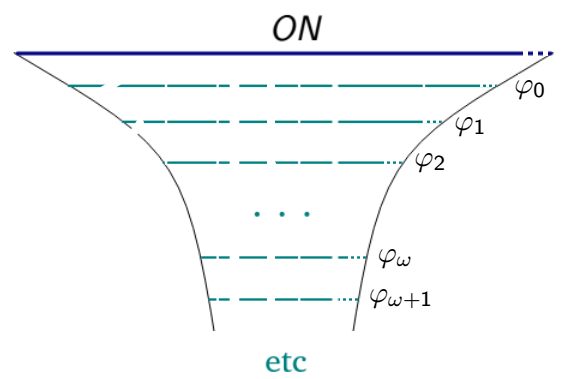
\includegraphics[scale=0.4]{veblen.png}
\caption{The range (image) of the first Veblen functions. Not on scale}
\end{figure}

\begin{itemize}
	\item Zero ordinal: $\varphi_0(\alpha) := \omega^\alpha$
	\item Successor ordinals $\rho$: $\varphi_{\rho+1}(\alpha) := Enum_{FIX\mathlarger{(}\varphi(\rho)\mathlarger{)}} (\alpha)$
	\item Limit ordinals $\lambda$: $\varphi_{\lambda}(\alpha) := Enum_{FIX\mathlarger{(}\displaystyle\cap_{\rho < \lambda}\varphi(\rho)\mathlarger{)}}(\alpha)$
\end{itemize} \pause

Remark: if $\rho_1 < \rho_2$ then $\varphi_{\rho_2}$ enumerates a subset of fixed points of $\varphi_{\rho_1}$

\end{frame}

\iffalse
\begin{frame}{Proof}

By induction in $\rho$: \pause

Case $\rho = 0:$

(...)

\end{frame}
\fi

\begin{frame}{Proof}

We want to prove that $\sintcons{\alpha}{\beta+\omega^\rho}\text{ implies }\sintcons{\phi_\rho(\alpha)}{\beta} \Delta$$ \pause

By induction on \(\rho\).

For \(\rho = 0\), we have \(\sintcons{\alpha}{\beta + \omega^0} = \sintcons{\alpha}{\beta +1}\).
By the Basic Elimination Theorem, we get
\(\sintcons{\omega^\alpha}{\beta}\Delta = \sintcons{\varphi_0(\alpha)}{\beta}\Delta\).

Now assume \(\rho > 0\). If the last inference was not a cut, we have,
$$
\sintcons{\alpha_\iota}{\beta+\omega^\rho} \Delta_\iota \text{for} \iota\in I \Rightarrow
\sintcons{\alpha}{\beta+\omega^\rho}\Delta
$$
with \(\alpha_\iota < \alpha\) for all \(\iota \in I\).

By the induction hypothesis, we get,
$$
\sintcons{\varphi_\rho(\alpha_\iota)}{\beta} \Delta_\iota \text{for} \iota\in I.
$$

Since for every \(\iota \in I\), \(\alpha_\iota < \alpha\), we have \(\varphi_\rho(\alpha_\iota) < \varphi_\rho(\alpha)\) (since the Veblen functions are strictly increasing). Thus, we get,
$$
\sintcons{\varphi_\rho(\alpha_\iota)}{\beta} \Delta_\iota \text{for} \iota\in I \Rightarrow
\sintcons{\varphi_\rho(\alpha)}{\beta}\Delta
$$
using the same inference.

Similarly, if the last inference was a cut of rank \(< \beta\), a similar argument
proves the statement.

\end{frame}

\begin{frame}{Proof (cont)}


Now assume that the last inference was
$$
\sintcons{\alpha_0}{\beta+\omega^\rho} \Delta, F \text{and}
\sintcons{\alpha_0}{\beta+\omega^\rho} \Delta, \neg F \Rightarrow
\sintcons{\alpha}{\beta+\omega^\rho}\Delta
$$
for \(\alpha_0 < \alpha\), and formula \(F\) such that \(rank(F) \in [\beta, \beta + \omega^\rho)\).

Let \(\gamma\) be an ordinal such that \(rank(F) = \beta + \gamma\). We decompose
\(\gamma\) into its Cantor Normal Form and get,
$$
rank(F) = \beta + \gamma = \beta + \omega^{\sigma_1} + ... + \omega^{\sigma_n}
< \beta + \omega^\rho
$$
such that \(\rho > \sigma_1 \geq \sigma_2 \geq ... \geq \sigma_n\), and thus,
$$
rank(F) < \beta + \omega^{\sigma_1}(n+1).
$$

We now do a side induction on \(\alpha\). When \(\alpha = 0\), the claim is trivial. Otherwise, we use the induction hypothesis to get,
$$
\sintcons{\varphi_\rho(\alpha_0)}{\beta} \Delta, F \text{and}
\sintcons{\varphi_\rho(\alpha_0)}{\beta} \Delta, \neg F.
$$
Thus, we get \(\sintcons{\varphi_\rho(\alpha_0)+1}{\beta + \omega^{\sigma_1}(n+1)} \Delta\) by a cut.

Since \(\sigma_1 < \rho\), we apply the induction hypothesis to get,
$$
\sintcons{\varphi_{\sigma_1}(\varphi_{\sigma_1}(...(\varphi_{\rho}(\alpha_0)+1)))}{\beta} \Delta =
\sintcons{\varphi_{\sigma_1}^{n+1}(\varphi_{\rho}(\alpha_0)+1)))}{\beta} \Delta
$$

\end{frame}

\begin{frame}{Claim}

Claim: $\varphi_{\sigma_1}^n(\varphi_\rho(\alpha_0)+1) < \varphi_\rho(\alpha)$ \pause


By induction on $n$. \pause

When $n=0, \varphi_{\sigma_1}^0(\varphi_\rho(\alpha_0)+1) = \varphi_\rho(\alpha_0)+1$ \pause  $< \varphi_\rho(\alpha)$. \pause

%"When n equals 0, this is just and the claim is trivially true

%Q: why is it true?
%A: Well just because the veblen functions grow faster than $\fomega$, which is not only strictly increasing but also increases an infinite amound each time. As \alpha_0 < \alpha, the image under \alpha will be much bigger than under \alpha_0 (in particular bigger than the succesor)

$n \Rightarrow n+1: \varphi_{\sigma_1}^{n+1}(\varphi_\rho(\alpha_0)+1) = \varphi_{\sigma_1}(\varphi_{\sigma_1}^n(\varphi_\rho(\alpha_0)+1))$ \pause

By I.H., this is less than  $\varphi_{\sigma_1}(\varphi_\rho(\alpha))$ and by definition this is equal to $\varphi_\rho(\alpha)$. \pause And we are done!

%Q: Why does that happen?

%A: Well the Veblen functions are defined inductively, remember? \phi_\rho just enumerates the fixed points of the previous one if \rho is a successor or the common fixed points of all the previous functions. In any case, as \sigma_1 is less than \rho, the range of $\phi_\rho$ will just be a subset of the fixed points of $\phi_{\sigma_1}. That's what we have the result.
\end{frame}

\iffalse


%TODO Hablar del elimination theorem

IN CONSTRUCTION
\begin{frame}

%$ {            \left( \sint \right)     _{\rho+1} ^{\alpha} }$  
%$\displaystyle \sint_{\rho+1}^{\alpha}$
%$\sint^{\alpha}_{\rho+1}$
If $\sint_{\rho+1}^{\alpha} \Delta$ then $\sint_{\rho}^{\omega^\alpha} \Delta$
\end{frame}

\begin{frame}{Idea of proof}
%TODO no mostra esta slide, pero quiero dejar escrita la idea...

\end{frame}

\begin{frame}{Predicative Elimination Lemma}
If $\sin_{\beta + \omega^\rho}^{\alpha} \Delta$ then $\sint_\beta{\phi_\rho(\alpha)} \Delta$

%TODO cambiar el width
%TODO tal vez hacer esta pregunta después de la demo? O justo antes
\begin{tcolorbox}
Why is it called predicative?
%\end{align}
\end{tcolorbox}
% Es porque mantenemos la predicatividad porque pagamos el costo de las veblen functions?
\end{frame}

\begin{frame}{Veblen function properties}
Acá hago el dibujo del cuerno de Gabriel con agujeritos. [NOT ON SCALE. Also in reality there are more holes. ] %TODO se dice así, NOT ON SCALE?

Veblen functions are defined inductively, $\phi_0$ and enumeration of fixed points of previous function.

They can be used to defined an ordinal notation system that extends the Cantor Normal Form notation (but of course only reach to a certain point ($\Gamma_0$) of the countable ordinals, as these are uncountable).

\end{frame}

\begin{frame}
Test:

\end{frame}



\begin{frame}{Proof}



By induction on $\rho$ and side induction in $\alpha$ % That means...

For $\rho=0$ we get BLA because $\phi_0 = \fomega$ \pause

So assume $\rho > 0$ % This is the main inductive step

If the last step was a cut of order less than $\beta$ entonces puedo aplicar la hipótesis inductiva a $\sint^{\alpha_0}_{\beta + \omega^\rho} \Delta, F, \sint^{\alpha_0}_{\beta + \omega^\rho} \Delta, \not F$ separately and get $\sint^{\phi_\rho(\alpha_0)}_{\beta } \Delta, F, \sint^{\phi_\rho(\alpha_0)}_{\beta } \Delta, \not F$, and then by a cut I get $\sint^{\phi_\rho(\alpha_0)}_{\beta } \Delta$ and this is less than $\sint^{\phi_\rho(\alpha)}_{\beta } \Delta$ because the $\phi$ functions are order preserving.


\end{frame}

\begin{frame}
\begin{tcolorbox}
Do we really need this?
\end{tcolorbox}

Answer: not here, but yes in other languages...
\end{frame}

\begin{frame}
	$$\varphi_0 = Enum_{\fomega}$$
	$$\varphi_1 = Enum_{Fix(\varphi_0)}$$
	$$\varphi_2 = Enum_{Fix(\varphi_1)}$$
	$$...$$
	$$\varphi_\omega = Enum_{ \displaystyle \cap_{i < \omega} Fix(\varphi_i)}$$
	$$\varphi_{\omega+1} = Enum_{Fix(\varphi_\omega)}$$
	$$ON$$
\end{frame}



\begin{frame}
\begin{tcolorbox}
%blablabla
\begin{align}
E &= mc^2 & \text{Formula of the universe}
\end{align}
Hoaray
\end{tcolorbox}

\end{frame}

\begin{frame}
	Theorem
\end{frame}

Q: Why do we need it? We can only take finite disjunctions.
A: Consider for example $L_\infty(NT)$, see p37 \url{https://www.uni-muenster.de/imperia/md/content/logik/Skripte/pohlers._infinitary_proof_theory.pdf}


\begin{frame}
	So what are we proving
\end{frame}

\begin{frame}
	Oh ok let's try induction on ordinals
\end{frame}

\begin{frame}
	Conclusions? So what's the nice thing about not having cuts?
	Preguntarle a Pohlers si esto sirve acá porque los cuts son finitos.
\end{frame}


\begin{frame}
\begin{tcolorbox}
blablabla
\begin{align}
E &= mc^2 & \text{Formula of the universe}
\end{align}
Hoaray
\end{tcolorbox}
\end{frame}

Veblen functions eat up other functions with lower subindices (da un menor o igual)
\fi
\end{document}